\documentclass[twoside]{book}

% Packages required by doxygen
\usepackage{fixltx2e}
\usepackage{calc}
\usepackage{doxygen}
\usepackage[export]{adjustbox} % also loads graphicx
\usepackage{graphicx}
\usepackage[utf8]{inputenc}
\usepackage{makeidx}
\usepackage{multicol}
\usepackage{multirow}
\PassOptionsToPackage{warn}{textcomp}
\usepackage{textcomp}
\usepackage[nointegrals]{wasysym}
\usepackage[table]{xcolor}

% Font selection
\usepackage[T1]{fontenc}
\usepackage[scaled=.90]{helvet}
\usepackage{courier}
\usepackage{amssymb}
\usepackage{sectsty}
\renewcommand{\familydefault}{\sfdefault}
\allsectionsfont{%
  \fontseries{bc}\selectfont%
  \color{darkgray}%
}
\renewcommand{\DoxyLabelFont}{%
  \fontseries{bc}\selectfont%
  \color{darkgray}%
}
\newcommand{\+}{\discretionary{\mbox{\scriptsize$\hookleftarrow$}}{}{}}

% Page & text layout
\usepackage{geometry}
\geometry{%
  a4paper,%
  top=2.5cm,%
  bottom=2.5cm,%
  left=2.5cm,%
  right=2.5cm%
}
\tolerance=750
\hfuzz=15pt
\hbadness=750
\setlength{\emergencystretch}{15pt}
\setlength{\parindent}{0cm}
\setlength{\parskip}{3ex plus 2ex minus 2ex}
\makeatletter
\renewcommand{\paragraph}{%
  \@startsection{paragraph}{4}{0ex}{-1.0ex}{1.0ex}{%
    \normalfont\normalsize\bfseries\SS@parafont%
  }%
}
\renewcommand{\subparagraph}{%
  \@startsection{subparagraph}{5}{0ex}{-1.0ex}{1.0ex}{%
    \normalfont\normalsize\bfseries\SS@subparafont%
  }%
}
\makeatother

% Headers & footers
\usepackage{fancyhdr}
\pagestyle{fancyplain}
\fancyhead[LE]{\fancyplain{}{\bfseries\thepage}}
\fancyhead[CE]{\fancyplain{}{}}
\fancyhead[RE]{\fancyplain{}{\bfseries\leftmark}}
\fancyhead[LO]{\fancyplain{}{\bfseries\rightmark}}
\fancyhead[CO]{\fancyplain{}{}}
\fancyhead[RO]{\fancyplain{}{\bfseries\thepage}}
\fancyfoot[LE]{\fancyplain{}{}}
\fancyfoot[CE]{\fancyplain{}{}}
\fancyfoot[RE]{\fancyplain{}{\bfseries\scriptsize Generated by Doxygen }}
\fancyfoot[LO]{\fancyplain{}{\bfseries\scriptsize Generated by Doxygen }}
\fancyfoot[CO]{\fancyplain{}{}}
\fancyfoot[RO]{\fancyplain{}{}}
\renewcommand{\footrulewidth}{0.4pt}
\renewcommand{\chaptermark}[1]{%
  \markboth{#1}{}%
}
\renewcommand{\sectionmark}[1]{%
  \markright{\thesection\ #1}%
}

% Indices & bibliography
\usepackage{natbib}
\usepackage[titles]{tocloft}
\setcounter{tocdepth}{3}
\setcounter{secnumdepth}{5}
\makeindex

% Hyperlinks (required, but should be loaded last)
\usepackage{ifpdf}
\ifpdf
  \usepackage[pdftex,pagebackref=true]{hyperref}
\else
  \usepackage[ps2pdf,pagebackref=true]{hyperref}
\fi
\hypersetup{%
  colorlinks=true,%
  linkcolor=blue,%
  citecolor=blue,%
  unicode%
}

% Custom commands
\newcommand{\clearemptydoublepage}{%
  \newpage{\pagestyle{empty}\cleardoublepage}%
}

\usepackage{caption}
\captionsetup{labelsep=space,justification=centering,font={bf},singlelinecheck=off,skip=4pt,position=top}

%===== C O N T E N T S =====

\begin{document}

% Titlepage & ToC
\hypersetup{pageanchor=false,
             bookmarksnumbered=true,
             pdfencoding=unicode
            }
\pagenumbering{alph}
\begin{titlepage}
\vspace*{7cm}
\begin{center}%
{\Large Server Node -\/ forecast project \\[1ex]\large 1 }\\
\vspace*{1cm}
{\large Generated by Doxygen 1.8.14}\\
\end{center}
\end{titlepage}
\clearemptydoublepage
\pagenumbering{roman}
\tableofcontents
\clearemptydoublepage
\pagenumbering{arabic}
\hypersetup{pageanchor=true}

%--- Begin generated contents ---
\chapter{Hierarchical Index}
\section{Class Hierarchy}
This inheritance list is sorted roughly, but not completely, alphabetically\+:\begin{DoxyCompactList}
\item \contentsline{section}{Clients}{\pageref{class_clients}}{}
\item \contentsline{section}{Data\+\_\+\+Converter}{\pageref{class_data___converter}}{}
\item \contentsline{section}{Data\+\_\+\+Parser\+\_\+\+And\+\_\+\+Converter}{\pageref{class_data___parser___and___converter}}{}
\item \contentsline{section}{Data\+\_\+\+Parser\+\_\+\+And\+\_\+\+Converter\+\_\+\+Tests}{\pageref{class_data___parser___and___converter___tests}}{}
\item \contentsline{section}{Network\+\_\+abstract}{\pageref{class_network__abstract}}{}
\begin{DoxyCompactList}
\item \contentsline{section}{Socket\+\_\+\+Communication}{\pageref{class_socket___communication}}{}
\end{DoxyCompactList}
\item \contentsline{section}{Sensor}{\pageref{class_sensor}}{}
\begin{DoxyCompactList}
\item \contentsline{section}{Temperature\+\_\+\+Sensor}{\pageref{class_temperature___sensor}}{}
\end{DoxyCompactList}
\item \contentsline{section}{Temperature\+\_\+\+Sensor\+\_\+\+Tests}{\pageref{class_temperature___sensor___tests}}{}
\end{DoxyCompactList}

\chapter{Class Index}
\section{Class List}
Here are the classes, structs, unions and interfaces with brief descriptions\+:\begin{DoxyCompactList}
\item\contentsline{section}{\mbox{\hyperlink{class_application___functions___tests}{Application\+\_\+\+Functions\+\_\+\+Tests}} }{\pageref{class_application___functions___tests}}{}
\item\contentsline{section}{\mbox{\hyperlink{class_data___parser___and___converter}{Data\+\_\+\+Parser\+\_\+\+And\+\_\+\+Converter}} }{\pageref{class_data___parser___and___converter}}{}
\item\contentsline{section}{\mbox{\hyperlink{class_data___parser___and___converter___tests}{Data\+\_\+\+Parser\+\_\+\+And\+\_\+\+Converter\+\_\+\+Tests}} }{\pageref{class_data___parser___and___converter___tests}}{}
\item\contentsline{section}{\mbox{\hyperlink{class_network__abstract}{Network\+\_\+abstract}} }{\pageref{class_network__abstract}}{}
\item\contentsline{section}{\mbox{\hyperlink{class_sensor}{Sensor}} }{\pageref{class_sensor}}{}
\item\contentsline{section}{\mbox{\hyperlink{class_socket___communication}{Socket\+\_\+\+Communication}} }{\pageref{class_socket___communication}}{}
\item\contentsline{section}{\mbox{\hyperlink{class_temperature___sensor}{Temperature\+\_\+\+Sensor}} }{\pageref{class_temperature___sensor}}{}
\item\contentsline{section}{\mbox{\hyperlink{class_temperature___server___tests}{Temperature\+\_\+\+Server\+\_\+\+Tests}} }{\pageref{class_temperature___server___tests}}{}
\end{DoxyCompactList}

\chapter{Class Documentation}
\hypertarget{class_application___functions___tests}{}\section{Application\+\_\+\+Functions\+\_\+\+Tests Class Reference}
\label{class_application___functions___tests}\index{Application\+\_\+\+Functions\+\_\+\+Tests@{Application\+\_\+\+Functions\+\_\+\+Tests}}


The documentation for this class was generated from the following files\+:\begin{DoxyCompactItemize}
\item 
D\+:/\+Dell Task/\+Client-\/\+Side/Application\+\_\+\+Functions\+\_\+\+Tests.\+h\item 
D\+:/\+Dell Task/\+Client-\/\+Side/Application\+\_\+\+Functions\+\_\+\+Tests.\+cpp\end{DoxyCompactItemize}

\hypertarget{class_data___parser___and___converter}{}\section{Data\+\_\+\+Parser\+\_\+\+And\+\_\+\+Converter Class Reference}
\label{class_data___parser___and___converter}\index{Data\+\_\+\+Parser\+\_\+\+And\+\_\+\+Converter@{Data\+\_\+\+Parser\+\_\+\+And\+\_\+\+Converter}}
\subsection*{Public Member Functions}
\begin{DoxyCompactItemize}
\item 
\mbox{\hyperlink{class_data___parser___and___converter_a6be39bded0dc784a018cca7228c5a400}{Data\+\_\+\+Parser\+\_\+\+And\+\_\+\+Converter}} ()
\end{DoxyCompactItemize}
\subsection*{Static Public Member Functions}
\begin{DoxyCompactItemize}
\item 
static std\+::map$<$ std\+::string, std\+::string $>$ \mbox{\hyperlink{class_data___parser___and___converter_a42e1a74db4715d980b83f42d103c25e2}{parse\+Data\+Then\+Convert\+To\+Map}} (std\+::string delimiter, std\+::string key\+Value\+Delimiter, std\+::string raw\+Data)
\item 
static std\+::pair$<$ std\+::string, std\+::string $>$ \mbox{\hyperlink{class_data___parser___and___converter_af44ead8fe2769d136227e3f603d14f70}{parse\+Data\+Then\+Convert\+To\+Pair}} (std\+::string delimiter, std\+::string raw\+Data)
\item 
static std\+::vector$<$ std\+::string $>$ \mbox{\hyperlink{class_data___parser___and___converter_aba2bbb38e79306b1da28ec1042e2b888}{parse\+Data\+Then\+Convert\+To\+Vector}} (std\+::string delimiter, std\+::string raw\+Data)
\end{DoxyCompactItemize}


\subsection{Constructor \& Destructor Documentation}
\mbox{\Hypertarget{class_data___parser___and___converter_a6be39bded0dc784a018cca7228c5a400}\label{class_data___parser___and___converter_a6be39bded0dc784a018cca7228c5a400}} 
\index{Data\+\_\+\+Parser\+\_\+\+And\+\_\+\+Converter@{Data\+\_\+\+Parser\+\_\+\+And\+\_\+\+Converter}!Data\+\_\+\+Parser\+\_\+\+And\+\_\+\+Converter@{Data\+\_\+\+Parser\+\_\+\+And\+\_\+\+Converter}}
\index{Data\+\_\+\+Parser\+\_\+\+And\+\_\+\+Converter@{Data\+\_\+\+Parser\+\_\+\+And\+\_\+\+Converter}!Data\+\_\+\+Parser\+\_\+\+And\+\_\+\+Converter@{Data\+\_\+\+Parser\+\_\+\+And\+\_\+\+Converter}}
\subsubsection{\texorpdfstring{Data\+\_\+\+Parser\+\_\+\+And\+\_\+\+Converter()}{Data\_Parser\_And\_Converter()}}
{\footnotesize\ttfamily Data\+\_\+\+Parser\+\_\+\+And\+\_\+\+Converter\+::\+Data\+\_\+\+Parser\+\_\+\+And\+\_\+\+Converter (\begin{DoxyParamCaption}{ }\end{DoxyParamCaption})}







\subsection{Member Function Documentation}
\mbox{\Hypertarget{class_data___parser___and___converter_a42e1a74db4715d980b83f42d103c25e2}\label{class_data___parser___and___converter_a42e1a74db4715d980b83f42d103c25e2}} 
\index{Data\+\_\+\+Parser\+\_\+\+And\+\_\+\+Converter@{Data\+\_\+\+Parser\+\_\+\+And\+\_\+\+Converter}!parse\+Data\+Then\+Convert\+To\+Map@{parse\+Data\+Then\+Convert\+To\+Map}}
\index{parse\+Data\+Then\+Convert\+To\+Map@{parse\+Data\+Then\+Convert\+To\+Map}!Data\+\_\+\+Parser\+\_\+\+And\+\_\+\+Converter@{Data\+\_\+\+Parser\+\_\+\+And\+\_\+\+Converter}}
\subsubsection{\texorpdfstring{parse\+Data\+Then\+Convert\+To\+Map()}{parseDataThenConvertToMap()}}
{\footnotesize\ttfamily std\+::map$<$ std\+::string, std\+::string $>$ Data\+\_\+\+Parser\+\_\+\+And\+\_\+\+Converter\+::parse\+Data\+Then\+Convert\+To\+Map (\begin{DoxyParamCaption}\item[{std\+::string}]{delimiter,  }\item[{std\+::string}]{key\+Value\+Delimiter,  }\item[{std\+::string}]{raw\+Data }\end{DoxyParamCaption})\hspace{0.3cm}{\ttfamily [static]}}






\begin{DoxyParams}{Parameters}
{\em delimiter} & \\
\hline
{\em key\+Value\+Delimiter} & \\
\hline
{\em raw\+Data} & \\
\hline
\end{DoxyParams}
\begin{DoxyReturn}{Returns}

\end{DoxyReturn}
\mbox{\Hypertarget{class_data___parser___and___converter_af44ead8fe2769d136227e3f603d14f70}\label{class_data___parser___and___converter_af44ead8fe2769d136227e3f603d14f70}} 
\index{Data\+\_\+\+Parser\+\_\+\+And\+\_\+\+Converter@{Data\+\_\+\+Parser\+\_\+\+And\+\_\+\+Converter}!parse\+Data\+Then\+Convert\+To\+Pair@{parse\+Data\+Then\+Convert\+To\+Pair}}
\index{parse\+Data\+Then\+Convert\+To\+Pair@{parse\+Data\+Then\+Convert\+To\+Pair}!Data\+\_\+\+Parser\+\_\+\+And\+\_\+\+Converter@{Data\+\_\+\+Parser\+\_\+\+And\+\_\+\+Converter}}
\subsubsection{\texorpdfstring{parse\+Data\+Then\+Convert\+To\+Pair()}{parseDataThenConvertToPair()}}
{\footnotesize\ttfamily std\+::pair$<$ std\+::string, std\+::string $>$ Data\+\_\+\+Parser\+\_\+\+And\+\_\+\+Converter\+::parse\+Data\+Then\+Convert\+To\+Pair (\begin{DoxyParamCaption}\item[{std\+::string}]{delimiter,  }\item[{std\+::string}]{raw\+Data }\end{DoxyParamCaption})\hspace{0.3cm}{\ttfamily [static]}}






\begin{DoxyParams}{Parameters}
{\em delimiter} & \\
\hline
{\em raw\+Data} & \\
\hline
\end{DoxyParams}
\begin{DoxyReturn}{Returns}

\end{DoxyReturn}
\mbox{\Hypertarget{class_data___parser___and___converter_aba2bbb38e79306b1da28ec1042e2b888}\label{class_data___parser___and___converter_aba2bbb38e79306b1da28ec1042e2b888}} 
\index{Data\+\_\+\+Parser\+\_\+\+And\+\_\+\+Converter@{Data\+\_\+\+Parser\+\_\+\+And\+\_\+\+Converter}!parse\+Data\+Then\+Convert\+To\+Vector@{parse\+Data\+Then\+Convert\+To\+Vector}}
\index{parse\+Data\+Then\+Convert\+To\+Vector@{parse\+Data\+Then\+Convert\+To\+Vector}!Data\+\_\+\+Parser\+\_\+\+And\+\_\+\+Converter@{Data\+\_\+\+Parser\+\_\+\+And\+\_\+\+Converter}}
\subsubsection{\texorpdfstring{parse\+Data\+Then\+Convert\+To\+Vector()}{parseDataThenConvertToVector()}}
{\footnotesize\ttfamily std\+::vector$<$ std\+::string $>$ Data\+\_\+\+Parser\+\_\+\+And\+\_\+\+Converter\+::parse\+Data\+Then\+Convert\+To\+Vector (\begin{DoxyParamCaption}\item[{std\+::string}]{delimiter,  }\item[{std\+::string}]{raw\+Data }\end{DoxyParamCaption})\hspace{0.3cm}{\ttfamily [static]}}






\begin{DoxyParams}{Parameters}
{\em delimiter} & \\
\hline
{\em raw\+Data} & \\
\hline
\end{DoxyParams}
\begin{DoxyReturn}{Returns}

\end{DoxyReturn}


The documentation for this class was generated from the following files\+:\begin{DoxyCompactItemize}
\item 
D\+:/\+Dell Task/\+Server-\/\+Side/Data\+\_\+\+Parser\+\_\+\+And\+\_\+\+Converter.\+h\item 
D\+:/\+Dell Task/\+Server-\/\+Side/Data\+\_\+\+Parser\+\_\+\+And\+\_\+\+Converter.\+cpp\end{DoxyCompactItemize}

\hypertarget{class_data___parser___and___converter___tests}{}\section{Data\+\_\+\+Parser\+\_\+\+And\+\_\+\+Converter\+\_\+\+Tests Class Reference}
\label{class_data___parser___and___converter___tests}\index{Data\+\_\+\+Parser\+\_\+\+And\+\_\+\+Converter\+\_\+\+Tests@{Data\+\_\+\+Parser\+\_\+\+And\+\_\+\+Converter\+\_\+\+Tests}}


The documentation for this class was generated from the following files\+:\begin{DoxyCompactItemize}
\item 
D\+:/\+Dell Task/\+Server-\/\+Side/Data\+\_\+\+Parser\+\_\+\+And\+\_\+\+Converter\+\_\+\+Tests.\+h\item 
D\+:/\+Dell Task/\+Server-\/\+Side/Data\+\_\+\+Parser\+\_\+\+And\+\_\+\+Converter\+\_\+\+Tests.\+cpp\end{DoxyCompactItemize}

\hypertarget{class_network__abstract}{}\section{Network\+\_\+abstract Class Reference}
\label{class_network__abstract}\index{Network\+\_\+abstract@{Network\+\_\+abstract}}
Inheritance diagram for Network\+\_\+abstract\+:\begin{figure}[H]
\begin{center}
\leavevmode
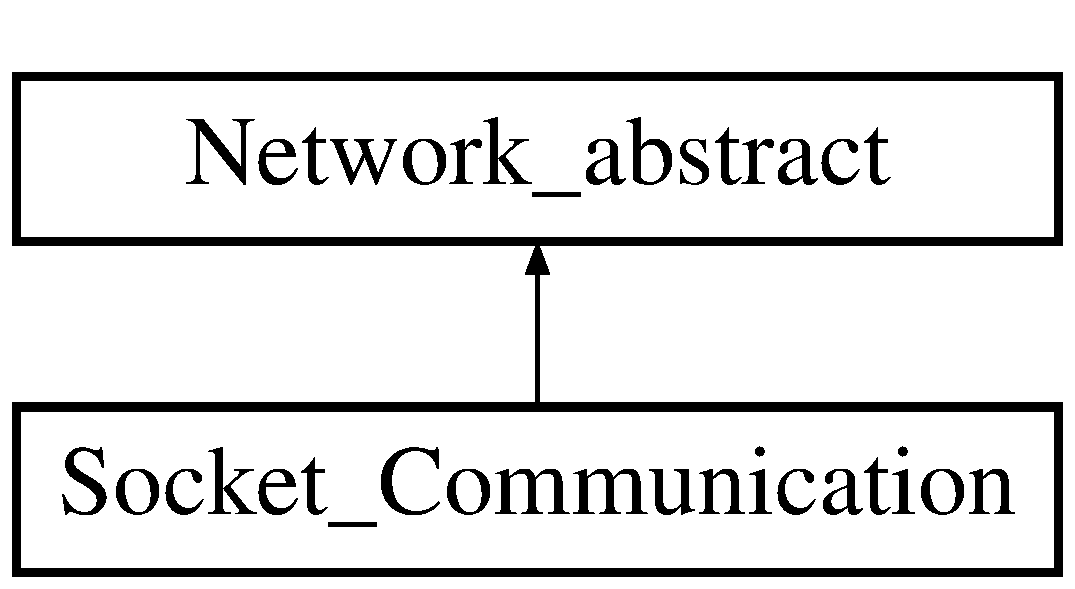
\includegraphics[height=2.000000cm]{class_network__abstract}
\end{center}
\end{figure}
\subsection*{Public Member Functions}
\begin{DoxyCompactItemize}
\item 
\mbox{\hyperlink{class_network__abstract_ada3172f8190180cbf9be59b2fd0450c3}{Network\+\_\+abstract}} ()
\item 
\mbox{\Hypertarget{class_network__abstract_a67c01479a3d2abcc9e69667006fd1db8}\label{class_network__abstract_a67c01479a3d2abcc9e69667006fd1db8}} 
virtual bool {\bfseries establish\+Connection} (std\+::map$<$ std\+::string, std\+::string $>$ protocol\+Parameters)=0
\item 
\mbox{\Hypertarget{class_network__abstract_a0c20f830bac3ab698e777862a855d918}\label{class_network__abstract_a0c20f830bac3ab698e777862a855d918}} 
virtual bool {\bfseries get\+Payload\+From\+Network} ()=0
\item 
std\+::string \mbox{\hyperlink{class_network__abstract_a70a5435d01dca002738e44ac148a97b1}{get\+Payload}} ()
\item 
void \mbox{\hyperlink{class_network__abstract_ac5bcf2e989845790f648118b7f382391}{set\+Payload}} (std\+::string payload)
\end{DoxyCompactItemize}
\subsection*{Protected Attributes}
\begin{DoxyCompactItemize}
\item 
\mbox{\Hypertarget{class_network__abstract_a56ca3ed6ac9c2a0225ea2d0f42f6b03e}\label{class_network__abstract_a56ca3ed6ac9c2a0225ea2d0f42f6b03e}} 
std\+::string {\bfseries payload}
\end{DoxyCompactItemize}


\subsection{Constructor \& Destructor Documentation}
\mbox{\Hypertarget{class_network__abstract_ada3172f8190180cbf9be59b2fd0450c3}\label{class_network__abstract_ada3172f8190180cbf9be59b2fd0450c3}} 
\index{Network\+\_\+abstract@{Network\+\_\+abstract}!Network\+\_\+abstract@{Network\+\_\+abstract}}
\index{Network\+\_\+abstract@{Network\+\_\+abstract}!Network\+\_\+abstract@{Network\+\_\+abstract}}
\subsubsection{\texorpdfstring{Network\+\_\+abstract()}{Network\_abstract()}}
{\footnotesize\ttfamily Network\+\_\+abstract\+::\+Network\+\_\+abstract (\begin{DoxyParamCaption}{ }\end{DoxyParamCaption})}







\subsection{Member Function Documentation}
\mbox{\Hypertarget{class_network__abstract_a70a5435d01dca002738e44ac148a97b1}\label{class_network__abstract_a70a5435d01dca002738e44ac148a97b1}} 
\index{Network\+\_\+abstract@{Network\+\_\+abstract}!get\+Payload@{get\+Payload}}
\index{get\+Payload@{get\+Payload}!Network\+\_\+abstract@{Network\+\_\+abstract}}
\subsubsection{\texorpdfstring{get\+Payload()}{getPayload()}}
{\footnotesize\ttfamily std\+::string Network\+\_\+abstract\+::get\+Payload (\begin{DoxyParamCaption}{ }\end{DoxyParamCaption})}





\begin{DoxyReturn}{Returns}

\end{DoxyReturn}
\mbox{\Hypertarget{class_network__abstract_ac5bcf2e989845790f648118b7f382391}\label{class_network__abstract_ac5bcf2e989845790f648118b7f382391}} 
\index{Network\+\_\+abstract@{Network\+\_\+abstract}!set\+Payload@{set\+Payload}}
\index{set\+Payload@{set\+Payload}!Network\+\_\+abstract@{Network\+\_\+abstract}}
\subsubsection{\texorpdfstring{set\+Payload()}{setPayload()}}
{\footnotesize\ttfamily void Network\+\_\+abstract\+::set\+Payload (\begin{DoxyParamCaption}\item[{std\+::string}]{payload }\end{DoxyParamCaption})}






\begin{DoxyParams}{Parameters}
{\em payload} & \\
\hline
\end{DoxyParams}


The documentation for this class was generated from the following files\+:\begin{DoxyCompactItemize}
\item 
D\+:/\+Dell Task/\+Client-\/\+Side/Network\+\_\+abstract.\+h\item 
D\+:/\+Dell Task/\+Client-\/\+Side/Network\+\_\+abstract.\+cpp\end{DoxyCompactItemize}

\hypertarget{class_sensor}{}\section{Sensor Class Reference}
\label{class_sensor}\index{Sensor@{Sensor}}
Inheritance diagram for Sensor\+:\begin{figure}[H]
\begin{center}
\leavevmode
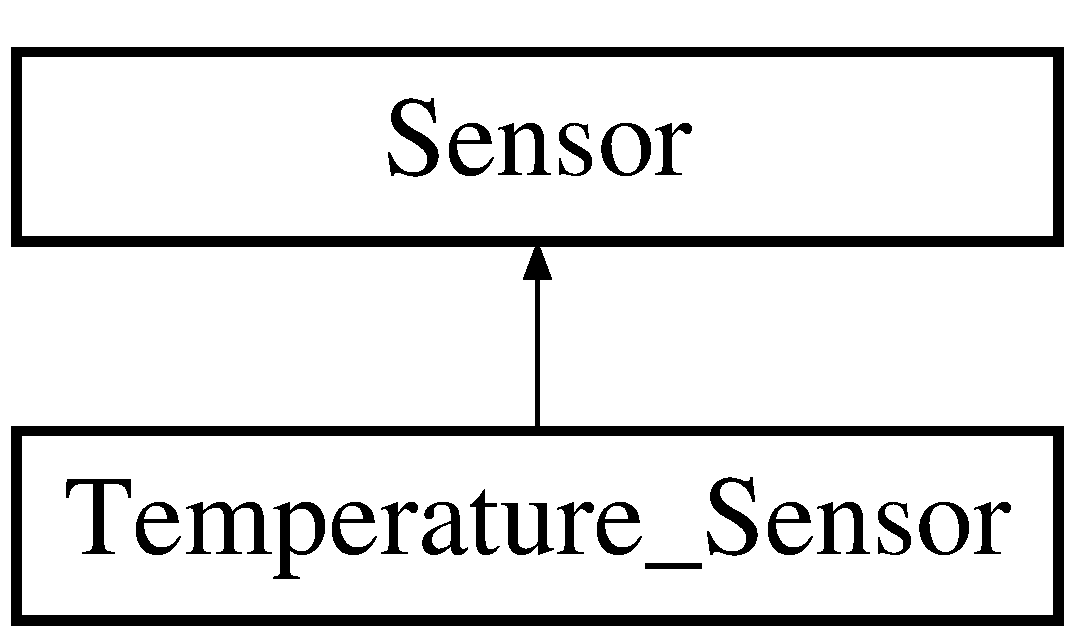
\includegraphics[height=2.000000cm]{class_sensor}
\end{center}
\end{figure}
\subsection*{Public Member Functions}
\begin{DoxyCompactItemize}
\item 
\mbox{\hyperlink{class_sensor_a342d6d11ef572c8cba92cb76fb1a294b}{Sensor}} ()
\item 
void \mbox{\hyperlink{class_sensor_add1838a85fc68b6c0b61a4a233e5fcaf}{set\+Sensor\+Name}} (std\+::string sensor\+Name)
\item 
std\+::string \mbox{\hyperlink{class_sensor_aa8250e5192cfd751fad294930fabf92b}{get\+Sensor\+Name}} ()
\item 
void \mbox{\hyperlink{class_sensor_a59ad3f638a81e29a9fac3526be948ce5}{set\+Sensor\+Serial\+Number}} (std\+::string sensor\+Type)
\item 
std\+::string \mbox{\hyperlink{class_sensor_ad59209d7c8aed356ba8aa2ff832c37cc}{get\+Sensor\+Serial\+Number}} ()
\item 
virtual void \mbox{\hyperlink{class_sensor_aa89b192e3203c85e62599c6239f01225}{set\+Sensor\+Reading}} (float sensor\+Reading)
\item 
float \mbox{\hyperlink{class_sensor_a399de2e826af7fe32a579f93dbfad1b2}{get\+Sensor\+Reading}} ()
\item 
void \mbox{\hyperlink{class_sensor_ab6e5cf0accf41d18ddb4dc9e489ba1ef}{set\+Sensor\+Last\+Reading\+Timestamp}} ()
\item 
tm \mbox{\hyperlink{class_sensor_a7a14fc550fd1c126f256925d07214d27}{get\+Sensor\+Last\+Reading\+Timestamp}} ()
\end{DoxyCompactItemize}
\subsection*{Protected Attributes}
\begin{DoxyCompactItemize}
\item 
\mbox{\Hypertarget{class_sensor_a636aa0945b0b99ccd71a02a8f552b9b5}\label{class_sensor_a636aa0945b0b99ccd71a02a8f552b9b5}} 
std\+::string {\bfseries sensor\+Name}
\item 
\mbox{\Hypertarget{class_sensor_abecc0caf1d4129a2da059ad3f28ed741}\label{class_sensor_abecc0caf1d4129a2da059ad3f28ed741}} 
std\+::string {\bfseries sensor\+Serial\+Number}
\item 
\mbox{\Hypertarget{class_sensor_ab83aea6e8f7690eb6abb6d30d97c5a94}\label{class_sensor_ab83aea6e8f7690eb6abb6d30d97c5a94}} 
std\+::string {\bfseries sensor\+Type}
\item 
\mbox{\Hypertarget{class_sensor_a3bfa0c158dc7e968bbb5990e031c7634}\label{class_sensor_a3bfa0c158dc7e968bbb5990e031c7634}} 
float {\bfseries sensor\+Reading}
\item 
\mbox{\Hypertarget{class_sensor_af94e2e6fe881a2be3d112f4c0b434090}\label{class_sensor_af94e2e6fe881a2be3d112f4c0b434090}} 
tm {\bfseries last\+Reading\+Time\+Stamp}
\end{DoxyCompactItemize}


\subsection{Constructor \& Destructor Documentation}
\mbox{\Hypertarget{class_sensor_a342d6d11ef572c8cba92cb76fb1a294b}\label{class_sensor_a342d6d11ef572c8cba92cb76fb1a294b}} 
\index{Sensor@{Sensor}!Sensor@{Sensor}}
\index{Sensor@{Sensor}!Sensor@{Sensor}}
\subsubsection{\texorpdfstring{Sensor()}{Sensor()}}
{\footnotesize\ttfamily Sensor\+::\+Sensor (\begin{DoxyParamCaption}{ }\end{DoxyParamCaption})}







\subsection{Member Function Documentation}
\mbox{\Hypertarget{class_sensor_a7a14fc550fd1c126f256925d07214d27}\label{class_sensor_a7a14fc550fd1c126f256925d07214d27}} 
\index{Sensor@{Sensor}!get\+Sensor\+Last\+Reading\+Timestamp@{get\+Sensor\+Last\+Reading\+Timestamp}}
\index{get\+Sensor\+Last\+Reading\+Timestamp@{get\+Sensor\+Last\+Reading\+Timestamp}!Sensor@{Sensor}}
\subsubsection{\texorpdfstring{get\+Sensor\+Last\+Reading\+Timestamp()}{getSensorLastReadingTimestamp()}}
{\footnotesize\ttfamily tm Sensor\+::get\+Sensor\+Last\+Reading\+Timestamp (\begin{DoxyParamCaption}{ }\end{DoxyParamCaption})}





\begin{DoxyReturn}{Returns}

\end{DoxyReturn}
\mbox{\Hypertarget{class_sensor_aa8250e5192cfd751fad294930fabf92b}\label{class_sensor_aa8250e5192cfd751fad294930fabf92b}} 
\index{Sensor@{Sensor}!get\+Sensor\+Name@{get\+Sensor\+Name}}
\index{get\+Sensor\+Name@{get\+Sensor\+Name}!Sensor@{Sensor}}
\subsubsection{\texorpdfstring{get\+Sensor\+Name()}{getSensorName()}}
{\footnotesize\ttfamily std\+::string Sensor\+::get\+Sensor\+Name (\begin{DoxyParamCaption}{ }\end{DoxyParamCaption})}





\begin{DoxyReturn}{Returns}

\end{DoxyReturn}
\mbox{\Hypertarget{class_sensor_a399de2e826af7fe32a579f93dbfad1b2}\label{class_sensor_a399de2e826af7fe32a579f93dbfad1b2}} 
\index{Sensor@{Sensor}!get\+Sensor\+Reading@{get\+Sensor\+Reading}}
\index{get\+Sensor\+Reading@{get\+Sensor\+Reading}!Sensor@{Sensor}}
\subsubsection{\texorpdfstring{get\+Sensor\+Reading()}{getSensorReading()}}
{\footnotesize\ttfamily float Sensor\+::get\+Sensor\+Reading (\begin{DoxyParamCaption}{ }\end{DoxyParamCaption})}





\begin{DoxyReturn}{Returns}

\end{DoxyReturn}
\mbox{\Hypertarget{class_sensor_ad59209d7c8aed356ba8aa2ff832c37cc}\label{class_sensor_ad59209d7c8aed356ba8aa2ff832c37cc}} 
\index{Sensor@{Sensor}!get\+Sensor\+Serial\+Number@{get\+Sensor\+Serial\+Number}}
\index{get\+Sensor\+Serial\+Number@{get\+Sensor\+Serial\+Number}!Sensor@{Sensor}}
\subsubsection{\texorpdfstring{get\+Sensor\+Serial\+Number()}{getSensorSerialNumber()}}
{\footnotesize\ttfamily std\+::string Sensor\+::get\+Sensor\+Serial\+Number (\begin{DoxyParamCaption}{ }\end{DoxyParamCaption})}





\begin{DoxyReturn}{Returns}

\end{DoxyReturn}
\mbox{\Hypertarget{class_sensor_ab6e5cf0accf41d18ddb4dc9e489ba1ef}\label{class_sensor_ab6e5cf0accf41d18ddb4dc9e489ba1ef}} 
\index{Sensor@{Sensor}!set\+Sensor\+Last\+Reading\+Timestamp@{set\+Sensor\+Last\+Reading\+Timestamp}}
\index{set\+Sensor\+Last\+Reading\+Timestamp@{set\+Sensor\+Last\+Reading\+Timestamp}!Sensor@{Sensor}}
\subsubsection{\texorpdfstring{set\+Sensor\+Last\+Reading\+Timestamp()}{setSensorLastReadingTimestamp()}}
{\footnotesize\ttfamily void Sensor\+::set\+Sensor\+Last\+Reading\+Timestamp (\begin{DoxyParamCaption}{ }\end{DoxyParamCaption})}





\mbox{\Hypertarget{class_sensor_add1838a85fc68b6c0b61a4a233e5fcaf}\label{class_sensor_add1838a85fc68b6c0b61a4a233e5fcaf}} 
\index{Sensor@{Sensor}!set\+Sensor\+Name@{set\+Sensor\+Name}}
\index{set\+Sensor\+Name@{set\+Sensor\+Name}!Sensor@{Sensor}}
\subsubsection{\texorpdfstring{set\+Sensor\+Name()}{setSensorName()}}
{\footnotesize\ttfamily void Sensor\+::set\+Sensor\+Name (\begin{DoxyParamCaption}\item[{std\+::string}]{sensor\+Name }\end{DoxyParamCaption})}






\begin{DoxyParams}{Parameters}
{\em sensor\+Name} & \\
\hline
\end{DoxyParams}
\mbox{\Hypertarget{class_sensor_aa89b192e3203c85e62599c6239f01225}\label{class_sensor_aa89b192e3203c85e62599c6239f01225}} 
\index{Sensor@{Sensor}!set\+Sensor\+Reading@{set\+Sensor\+Reading}}
\index{set\+Sensor\+Reading@{set\+Sensor\+Reading}!Sensor@{Sensor}}
\subsubsection{\texorpdfstring{set\+Sensor\+Reading()}{setSensorReading()}}
{\footnotesize\ttfamily void Sensor\+::set\+Sensor\+Reading (\begin{DoxyParamCaption}\item[{float}]{sensor\+Reading }\end{DoxyParamCaption})\hspace{0.3cm}{\ttfamily [virtual]}}






\begin{DoxyParams}{Parameters}
{\em sensor\+Reading} & \\
\hline
\end{DoxyParams}


Reimplemented in \mbox{\hyperlink{class_temperature___sensor_a9dcb003cce1faf22a5a22071ca95b2b4}{Temperature\+\_\+\+Sensor}}.

\mbox{\Hypertarget{class_sensor_a59ad3f638a81e29a9fac3526be948ce5}\label{class_sensor_a59ad3f638a81e29a9fac3526be948ce5}} 
\index{Sensor@{Sensor}!set\+Sensor\+Serial\+Number@{set\+Sensor\+Serial\+Number}}
\index{set\+Sensor\+Serial\+Number@{set\+Sensor\+Serial\+Number}!Sensor@{Sensor}}
\subsubsection{\texorpdfstring{set\+Sensor\+Serial\+Number()}{setSensorSerialNumber()}}
{\footnotesize\ttfamily void Sensor\+::set\+Sensor\+Serial\+Number (\begin{DoxyParamCaption}\item[{std\+::string}]{sensor\+Serial\+Number }\end{DoxyParamCaption})}






\begin{DoxyParams}{Parameters}
{\em sensor\+Serial\+Number} & \\
\hline
\end{DoxyParams}


The documentation for this class was generated from the following files\+:\begin{DoxyCompactItemize}
\item 
D\+:/\+Dell Task/\+Client-\/\+Side/Sensor.\+h\item 
D\+:/\+Dell Task/\+Client-\/\+Side/Sensor.\+cpp\end{DoxyCompactItemize}

\hypertarget{class_socket___communication}{}\section{Socket\+\_\+\+Communication Class Reference}
\label{class_socket___communication}\index{Socket\+\_\+\+Communication@{Socket\+\_\+\+Communication}}
Inheritance diagram for Socket\+\_\+\+Communication\+:\begin{figure}[H]
\begin{center}
\leavevmode
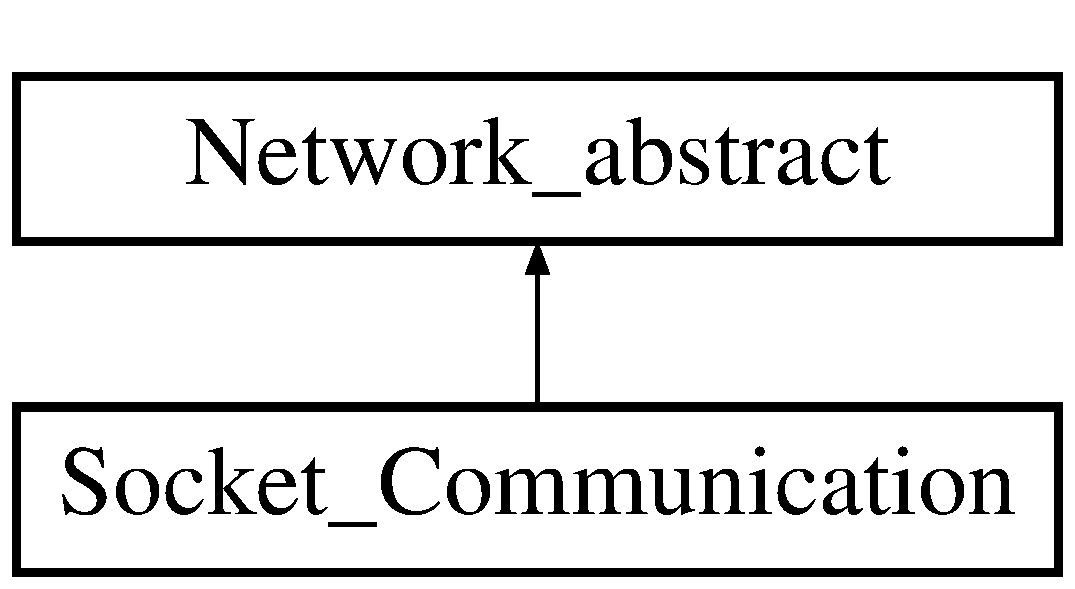
\includegraphics[height=2.000000cm]{class_socket___communication}
\end{center}
\end{figure}
\subsection*{Public Member Functions}
\begin{DoxyCompactItemize}
\item 
bool \mbox{\hyperlink{class_socket___communication_a238f29a5a991144d97caeabeadb34a93}{establish\+Connection}} ()
\item 
bool \mbox{\hyperlink{class_socket___communication_a7004e7ba47e3d78f2c497329b869d864}{send\+Payload\+Throw\+Network}} (std\+::map$<$ std\+::string, std\+::string $>$ protocol\+Parameters, std\+::string payload)
\end{DoxyCompactItemize}
\subsection*{Static Public Member Functions}
\begin{DoxyCompactItemize}
\item 
static \mbox{\hyperlink{class_socket___communication}{Socket\+\_\+\+Communication}} $\ast$ \mbox{\hyperlink{class_socket___communication_a7e156c8010a798636b637262adb1e38f}{get\+Inestance}} ()
\end{DoxyCompactItemize}
\subsection*{Additional Inherited Members}


\subsection{Member Function Documentation}
\mbox{\Hypertarget{class_socket___communication_a238f29a5a991144d97caeabeadb34a93}\label{class_socket___communication_a238f29a5a991144d97caeabeadb34a93}} 
\index{Socket\+\_\+\+Communication@{Socket\+\_\+\+Communication}!establish\+Connection@{establish\+Connection}}
\index{establish\+Connection@{establish\+Connection}!Socket\+\_\+\+Communication@{Socket\+\_\+\+Communication}}
\subsubsection{\texorpdfstring{establish\+Connection()}{establishConnection()}}
{\footnotesize\ttfamily bool Socket\+\_\+\+Communication\+::establish\+Connection (\begin{DoxyParamCaption}{ }\end{DoxyParamCaption})\hspace{0.3cm}{\ttfamily [virtual]}}





\begin{DoxyReturn}{Returns}

\end{DoxyReturn}


Implements \mbox{\hyperlink{class_network__abstract}{Network\+\_\+abstract}}.

\mbox{\Hypertarget{class_socket___communication_a7e156c8010a798636b637262adb1e38f}\label{class_socket___communication_a7e156c8010a798636b637262adb1e38f}} 
\index{Socket\+\_\+\+Communication@{Socket\+\_\+\+Communication}!get\+Inestance@{get\+Inestance}}
\index{get\+Inestance@{get\+Inestance}!Socket\+\_\+\+Communication@{Socket\+\_\+\+Communication}}
\subsubsection{\texorpdfstring{get\+Inestance()}{getInestance()}}
{\footnotesize\ttfamily \mbox{\hyperlink{class_socket___communication}{Socket\+\_\+\+Communication}} $\ast$ Socket\+\_\+\+Communication\+::get\+Inestance (\begin{DoxyParamCaption}{ }\end{DoxyParamCaption})\hspace{0.3cm}{\ttfamily [static]}}





\begin{DoxyReturn}{Returns}

\end{DoxyReturn}
\mbox{\Hypertarget{class_socket___communication_a7004e7ba47e3d78f2c497329b869d864}\label{class_socket___communication_a7004e7ba47e3d78f2c497329b869d864}} 
\index{Socket\+\_\+\+Communication@{Socket\+\_\+\+Communication}!send\+Payload\+Throw\+Network@{send\+Payload\+Throw\+Network}}
\index{send\+Payload\+Throw\+Network@{send\+Payload\+Throw\+Network}!Socket\+\_\+\+Communication@{Socket\+\_\+\+Communication}}
\subsubsection{\texorpdfstring{send\+Payload\+Throw\+Network()}{sendPayloadThrowNetwork()}}
{\footnotesize\ttfamily bool Socket\+\_\+\+Communication\+::send\+Payload\+Throw\+Network (\begin{DoxyParamCaption}\item[{std\+::map$<$ std\+::string, std\+::string $>$}]{protocol\+Parameters,  }\item[{std\+::string}]{payload }\end{DoxyParamCaption})\hspace{0.3cm}{\ttfamily [virtual]}}






\begin{DoxyParams}{Parameters}
{\em protocol\+Parameters} & \\
\hline
{\em payload} & \\
\hline
\end{DoxyParams}
\begin{DoxyReturn}{Returns}

\end{DoxyReturn}


Implements \mbox{\hyperlink{class_network__abstract}{Network\+\_\+abstract}}.



The documentation for this class was generated from the following files\+:\begin{DoxyCompactItemize}
\item 
D\+:/\+Dell Task/\+Server-\/\+Side/Socket\+\_\+\+Communication.\+h\item 
D\+:/\+Dell Task/\+Server-\/\+Side/Socket\+\_\+\+Communication.\+cpp\end{DoxyCompactItemize}

\hypertarget{class_temperature___sensor}{}\section{Temperature\+\_\+\+Sensor Class Reference}
\label{class_temperature___sensor}\index{Temperature\+\_\+\+Sensor@{Temperature\+\_\+\+Sensor}}
Inheritance diagram for Temperature\+\_\+\+Sensor\+:\begin{figure}[H]
\begin{center}
\leavevmode
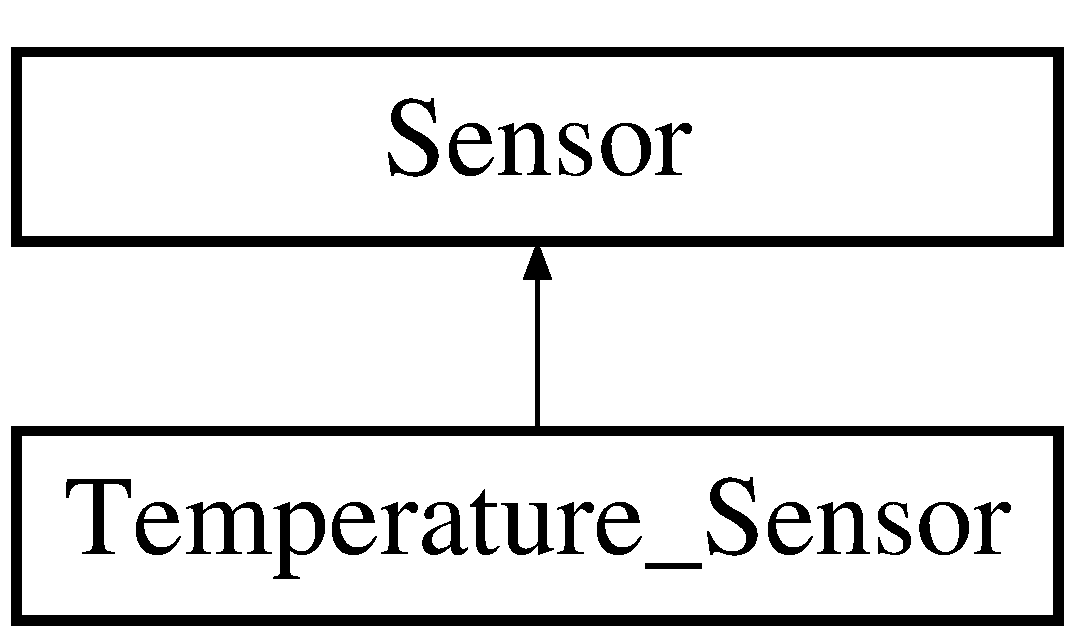
\includegraphics[height=2.000000cm]{class_temperature___sensor}
\end{center}
\end{figure}
\subsection*{Public Member Functions}
\begin{DoxyCompactItemize}
\item 
\mbox{\hyperlink{class_temperature___sensor_ab0f4f8edbe06c0829adf2913363c8ec6}{Temperature\+\_\+\+Sensor}} ()
\item 
void \mbox{\hyperlink{class_temperature___sensor_a14de6b8ba681b5720ff26113f99d8e45}{generate\+Temperature\+Periodically}} ()
\item 
float \mbox{\hyperlink{class_temperature___sensor_a6e12d531cd569ffcfa0a7ed0b2aeb6d0}{generate\+Temperature}} (int min, int max)
\end{DoxyCompactItemize}
\subsection*{Additional Inherited Members}


\subsection{Constructor \& Destructor Documentation}
\mbox{\Hypertarget{class_temperature___sensor_ab0f4f8edbe06c0829adf2913363c8ec6}\label{class_temperature___sensor_ab0f4f8edbe06c0829adf2913363c8ec6}} 
\index{Temperature\+\_\+\+Sensor@{Temperature\+\_\+\+Sensor}!Temperature\+\_\+\+Sensor@{Temperature\+\_\+\+Sensor}}
\index{Temperature\+\_\+\+Sensor@{Temperature\+\_\+\+Sensor}!Temperature\+\_\+\+Sensor@{Temperature\+\_\+\+Sensor}}
\subsubsection{\texorpdfstring{Temperature\+\_\+\+Sensor()}{Temperature\_Sensor()}}
{\footnotesize\ttfamily Temperature\+\_\+\+Sensor\+::\+Temperature\+\_\+\+Sensor (\begin{DoxyParamCaption}{ }\end{DoxyParamCaption})}







\subsection{Member Function Documentation}
\mbox{\Hypertarget{class_temperature___sensor_a6e12d531cd569ffcfa0a7ed0b2aeb6d0}\label{class_temperature___sensor_a6e12d531cd569ffcfa0a7ed0b2aeb6d0}} 
\index{Temperature\+\_\+\+Sensor@{Temperature\+\_\+\+Sensor}!generate\+Temperature@{generate\+Temperature}}
\index{generate\+Temperature@{generate\+Temperature}!Temperature\+\_\+\+Sensor@{Temperature\+\_\+\+Sensor}}
\subsubsection{\texorpdfstring{generate\+Temperature()}{generateTemperature()}}
{\footnotesize\ttfamily float Temperature\+\_\+\+Sensor\+::generate\+Temperature (\begin{DoxyParamCaption}\item[{int}]{min,  }\item[{int}]{max }\end{DoxyParamCaption})}






\begin{DoxyParams}{Parameters}
{\em min} & \\
\hline
{\em max} & \\
\hline
\end{DoxyParams}
\begin{DoxyReturn}{Returns}

\end{DoxyReturn}
\mbox{\Hypertarget{class_temperature___sensor_a14de6b8ba681b5720ff26113f99d8e45}\label{class_temperature___sensor_a14de6b8ba681b5720ff26113f99d8e45}} 
\index{Temperature\+\_\+\+Sensor@{Temperature\+\_\+\+Sensor}!generate\+Temperature\+Periodically@{generate\+Temperature\+Periodically}}
\index{generate\+Temperature\+Periodically@{generate\+Temperature\+Periodically}!Temperature\+\_\+\+Sensor@{Temperature\+\_\+\+Sensor}}
\subsubsection{\texorpdfstring{generate\+Temperature\+Periodically()}{generateTemperaturePeriodically()}}
{\footnotesize\ttfamily void Temperature\+\_\+\+Sensor\+::generate\+Temperature\+Periodically (\begin{DoxyParamCaption}{ }\end{DoxyParamCaption})}







The documentation for this class was generated from the following files\+:\begin{DoxyCompactItemize}
\item 
D\+:/\+Dell Task/\+Server-\/\+Side/Temperature\+\_\+\+Sensor.\+h\item 
D\+:/\+Dell Task/\+Server-\/\+Side/Temperature\+\_\+\+Sensor.\+cpp\end{DoxyCompactItemize}

\hypertarget{class_temperature___server___tests}{}\section{Temperature\+\_\+\+Server\+\_\+\+Tests Class Reference}
\label{class_temperature___server___tests}\index{Temperature\+\_\+\+Server\+\_\+\+Tests@{Temperature\+\_\+\+Server\+\_\+\+Tests}}
\subsection*{Public Member Functions}
\begin{DoxyCompactItemize}
\item 
\mbox{\hyperlink{class_temperature___server___tests_a2f79ed454ebd677befa6b0772cac7613}{Temperature\+\_\+\+Server\+\_\+\+Tests}} ()
\end{DoxyCompactItemize}


\subsection{Constructor \& Destructor Documentation}
\mbox{\Hypertarget{class_temperature___server___tests_a2f79ed454ebd677befa6b0772cac7613}\label{class_temperature___server___tests_a2f79ed454ebd677befa6b0772cac7613}} 
\index{Temperature\+\_\+\+Server\+\_\+\+Tests@{Temperature\+\_\+\+Server\+\_\+\+Tests}!Temperature\+\_\+\+Server\+\_\+\+Tests@{Temperature\+\_\+\+Server\+\_\+\+Tests}}
\index{Temperature\+\_\+\+Server\+\_\+\+Tests@{Temperature\+\_\+\+Server\+\_\+\+Tests}!Temperature\+\_\+\+Server\+\_\+\+Tests@{Temperature\+\_\+\+Server\+\_\+\+Tests}}
\subsubsection{\texorpdfstring{Temperature\+\_\+\+Server\+\_\+\+Tests()}{Temperature\_Server\_Tests()}}
{\footnotesize\ttfamily Temperature\+\_\+\+Server\+\_\+\+Tests\+::\+Temperature\+\_\+\+Server\+\_\+\+Tests (\begin{DoxyParamCaption}{ }\end{DoxyParamCaption})}







The documentation for this class was generated from the following files\+:\begin{DoxyCompactItemize}
\item 
D\+:/\+Dell Task/\+Client-\/\+Side/Temperature\+\_\+\+Server\+\_\+\+Tests.\+h\item 
D\+:/\+Dell Task/\+Client-\/\+Side/Temperature\+\_\+\+Server\+\_\+\+Tests.\+cpp\end{DoxyCompactItemize}

%--- End generated contents ---

% Index
\backmatter
\newpage
\phantomsection
\clearemptydoublepage
\addcontentsline{toc}{chapter}{Index}
\printindex

\end{document}
